\documentclass[a4paper,12pt]{article}

\usepackage[T1,T2A]{fontenc}
\usepackage[utf8]{inputenc}
\usepackage[utf8]{inputenc}
\usepackage[russian]{babel}
\usepackage{amsmath}
\usepackage{graphicx}
%\graphicspath{{/home/doktorkrab/code/lksh/vstup/prac}}
\begin{document}
\begin{enumerate}
\item \begin{enumerate}
\item Докажем, что вершина моста --- точка сочленения. Рассмотрим ребро $(v, u)$. Так как при удалении вершины $w$, удаляются все ребра, которые ведут в вершину $w$, то при удалении вершины $v$ или вершины $u$ удалится так же и ребро $(v,u)$, которое по условию является мостом, следовательно, компонента, содержащая $(v,u)$, распадется на новые компоненты, которые будут не пустые так как граф кубический, значит вершины $v$ и $u$ являются точками сочленения.
\item Докажем, что в кубическом графе не существует точки сочленения, которая не является вершиной моста. Доказывать будем от противного. Допустим существует точка сочленения $v$, которая не является мостом. Рассмотрим компоненты, на которые распадается компонента, которая содержит вершину $v$, после удаления вершины $v$. Должно быть не менее двух ребер, которые соединяют вершину $v$ и $i$-ую компоненту, так как иначе было бы единственное ребро --- мост ,и тогда вершина $v$ была бы одним из концов моста. Так как после удаления вершины $v$, компонента, содержащая эту вершину, распадается минимум на две компоненты, то степень вершины $v$ должна быть минимум 4, а по условию степень всех вершин в графе --- 3, мы пришли к противоречию, значит такой вершины не существует.
\end{enumerate}
\item Нет, можно привести пример:\\
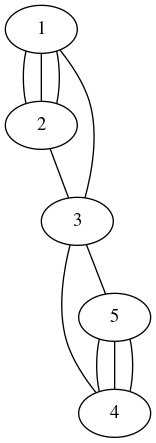
\includegraphics[scale=0.4]{test.png}\\
Здесь точка 3 является точкой сочленения, то при этом не является одним из концов моста.
\end{enumerate}
\end{document}